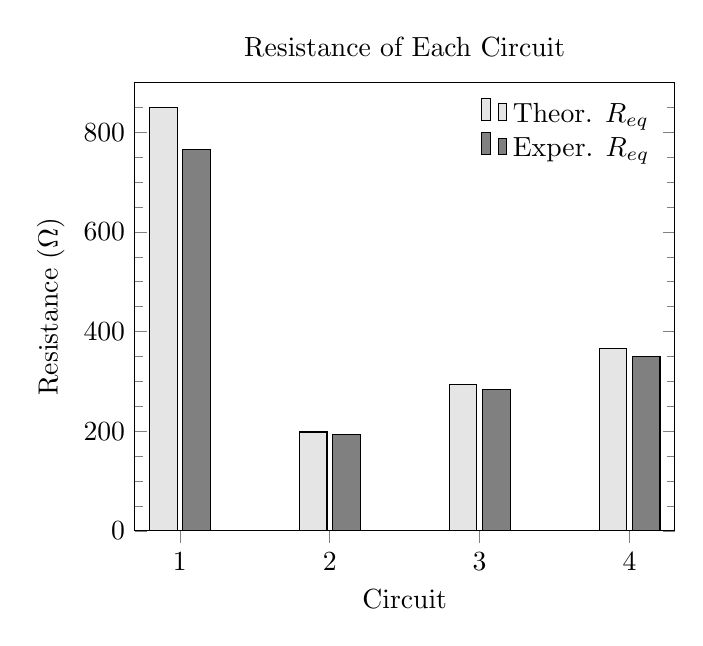
\begin{tikzpicture}

    \begin{axis}[
        xtick = { 1,...,4 },
        xtick pos = left,
        xticklabels = { 1, 2, 3, 4 },
        ymax = 900,
        ymin = 0,
        minor y tick num = 3,
        xlabel = { Circuit },
        ylabel = { Resistance ($\Omega$) },
        ybar,
        legend cell align = left,
        legend style = { draw = none },
        title = { Resistance of Each Circuit }
    ]
    
   	 	\addplot[
        		fill = black!10,
        		draw = black
        	]
        	table {
        		x  y      label
        		1  850.0  1
        		2  198.3  2
        		3  294.0  3
        		4  366.4  4
        	};
    
        \addplot[
            fill = black!50,
            draw = black
        ]
        table {
            x  y
            1  765.3
            2  193.3
            3  283.0
            4  350.5
        };
        
        \legend {
            Theor. $R_{eq}$,
            Exper. $R_{eq}$
        }
        
    \end{axis}

\end{tikzpicture}
